
\documentclass[10pt]{llncs}

\usepackage{cite}
\usepackage{mathptmx}
\usepackage{graphicx}
\usepackage{times}
%\usepackage{tabularx}
\usepackage{amsmath}
\usepackage{amsfonts}
%\usepackage{url}
\usepackage{caption}
\usepackage{multirow}
\usepackage{paralist}
\usepackage{listings}

\usepackage{color}
\definecolor{RED}{rgb}{1,0,0}
\definecolor{BLUE}{rgb}{0,0,1}
\newcommand{\FIXME}[1]{\textbf{\color{BLUE}{FIXME: #1}}}
\newcommand{\sref}[1]{Section~\ref{#1}}
\newcommand{\lref}[1]{Listing~\ref{#1}}
\newcommand{\fig}[1]{Figure~\ref{#1}}

% suppress  single floating lines on top (widow) and bottom (club)
%  10000 is infinity
%  tradeoff: possible underful vboxes
\clubpenalty=10000
\widowpenalty=10000

% correct bad hyphenation here
\hyphenation{op-tical net-works semi-conduc-tor}


\begin{document}
\lstset{language=[11]C++,basicstyle=\scriptsize,captionpos=b}
%
% paper title
% Titles are generally capitalized except for words such as a, an, and, as,
% at, but, by, for, in, nor, of, on, or, the, to and up, which are usually
% not capitalized unless they are the first or last word of the title.
% Linebreaks \\ can be used within to get better formatting as desired.
% Do not put math or special symbols in the title.
\title{From Big Data to Big Displays\\
High-Performance Visualization at Blue Brain}

%
%
% author names and IEEE memberships
% note positions of commas and nonbreaking spaces ( ~ ) LaTeX will not break
% a structure at a ~ so this keeps an author's name from being broken across
% two lines.
% use \thanks{} to gain access to the first footnote area
% a separate \thanks must be used for each paragraph as LaTeX2e's \thanks
% was not built to handle multiple paragraphs
%
%
%\IEEEcompsocitemizethanks is a special \thanks that produces the bulleted
% lists the Computer Society journals use for "first footnote" author
% affiliations. Use \IEEEcompsocthanksitem which works much like \item
% for each affiliation group. When not in compsoc mode,
% \IEEEcompsocitemizethanks becomes like \thanks and
% \IEEEcompsocthanksitem becomes a line break with idention. This
% facilitates dual compilation, although admittedly the differences in the
% desired content of \author between the different types of papers makes a
% one-size-fits-all approach a daunting prospect. For instance, compsoc
% journal papers have the author affiliations above the "Manuscript
% received ..."  text while in non-compsoc journals this is reversed. Sigh.

%% Author and Affiliation (multiple authors with multiple affiliations)
\author{Stefan~Eilemann, et.al.}
\institute{Blue Brain Project, Ecole Polytechnique Federale de Lausanne}

% make the title area
\maketitle


\begin{abstract}
  The Blue Brain project has been investing in high-performance visualization
  (HPV) to complement its HPC strategy since its inception in 2007. In 2011,
  this strategy has been accelerated to develop innovative visualization
  solutions through through increased funding and strategic partnerships with
  other research institutions.

  We present the key elements of this HPV ecosystem, which integrates C++
  visualization applications with novel collaborative display systems. We
  motivate how our strategy of transforming high-performance visualization
  engines into services enables a variety of use cases, not only for the
  integration with high-fidelity displays, but also to build service oriented
  architectures, to link into web applications and to provide remote services to
  python applications.
\end{abstract}

\section{Collaborative Displays}

Collaborative display systems are the integration point of the Blue Brain
visualization infrastructure. They are the evolution of existing visualization
systems. Compared to the current single-user or single-presenter systems,
collaborative display systems enable real team work through a combination of
size, resolution and user friendly implementation. Compared to immersive
visualization systems like the CAVE, they provide a simple to use environment
for high-fidelity visualization. For all use cases, the increased display size
and resolution allows improved data exploration for 2D and 3D content.

\subsection{Tiled Multitouch Display Walls}

The core of the Blue Brain visualization infrastructure are multiple
high-resolution tiled display walls driven by our Tide software~\cite{tide}. All
walls are equipped with a multitouch user interface and can be remote controlled
from any web browser. The walls are build using thin-bezel, 55 inch, Full HD LCD
panels with a hardened glass sheet. We use $4\times 3$ and $3\times 3$
configurations for a total of 24 and 18 Megapixel resolution, respectively. The
display size of over five meter diagonally (four meter for $3\times 3$) allows
team-size collaboration (up to ten people) or project-wide presentations (up to
a hundred people). \fig{fTDW} shows one wall during a project-wide presentation
with multiple interactive applications.

\begin{figure}[h!t]
  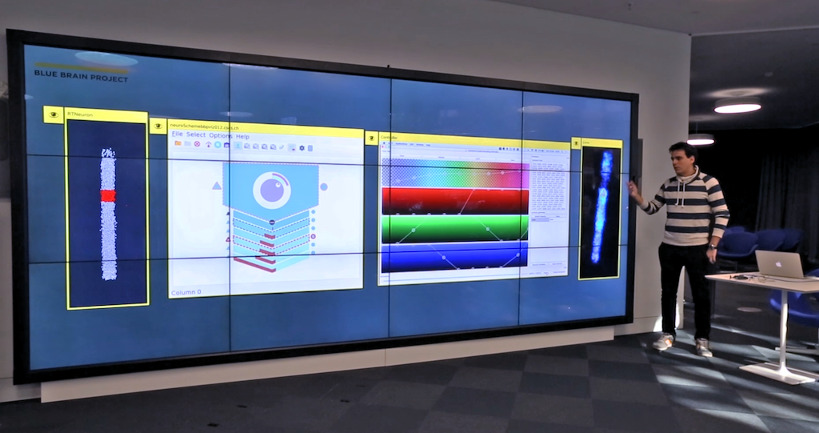
\includegraphics[width=\columnwidth]{images/tdw}
  \caption{\label{fTDW}Blue Brain $4\times 3$ tiled display wall}
\end{figure}

In the last years we created a production-ready setup of monoscopic tiled
display walls. On one hand, while there is substantial research on tiled display
wall software, we found that most solutions where not ready to be used in
$24\times 7$ unattained environment. On the other hand, the technology has been
commoditized to make these type of installations affordable to medium-sized
institutions which allowed us to build the software integration for a reasonable
startup cost. The multitouch user interface implements a low entry barrier for
new users, which is a unique capability of our solution.

\subsection{OpenDeck}

OpenDeck is our next-generation visualization system, aiming to integrate the
success of tiled display walls with a seamless transition to fully immersive
environments. We are currently in the process of installing the system which
consists of a semi-cylindrical back-projection screen with a 41 Megapixel usable
resolution on a 36 $m^2$ surface (\fig{fOpenDeck}). Like the display walls, it
is equipped with multitouch capabilities which makes it usable as a monoscopic
collaboration system from the first day of installations. Unlike tiled display
walls, it is active stereo capable and is equipped with a 3D tracking system for
immersive rendering. For increased immersion, a lower resolution front
projection system fills in the floor area. OpenDeck will allow us to run our
applications based on Equalizer~\cite{EMP:09} once the system is installed.

\begin{figure}[h!t]
  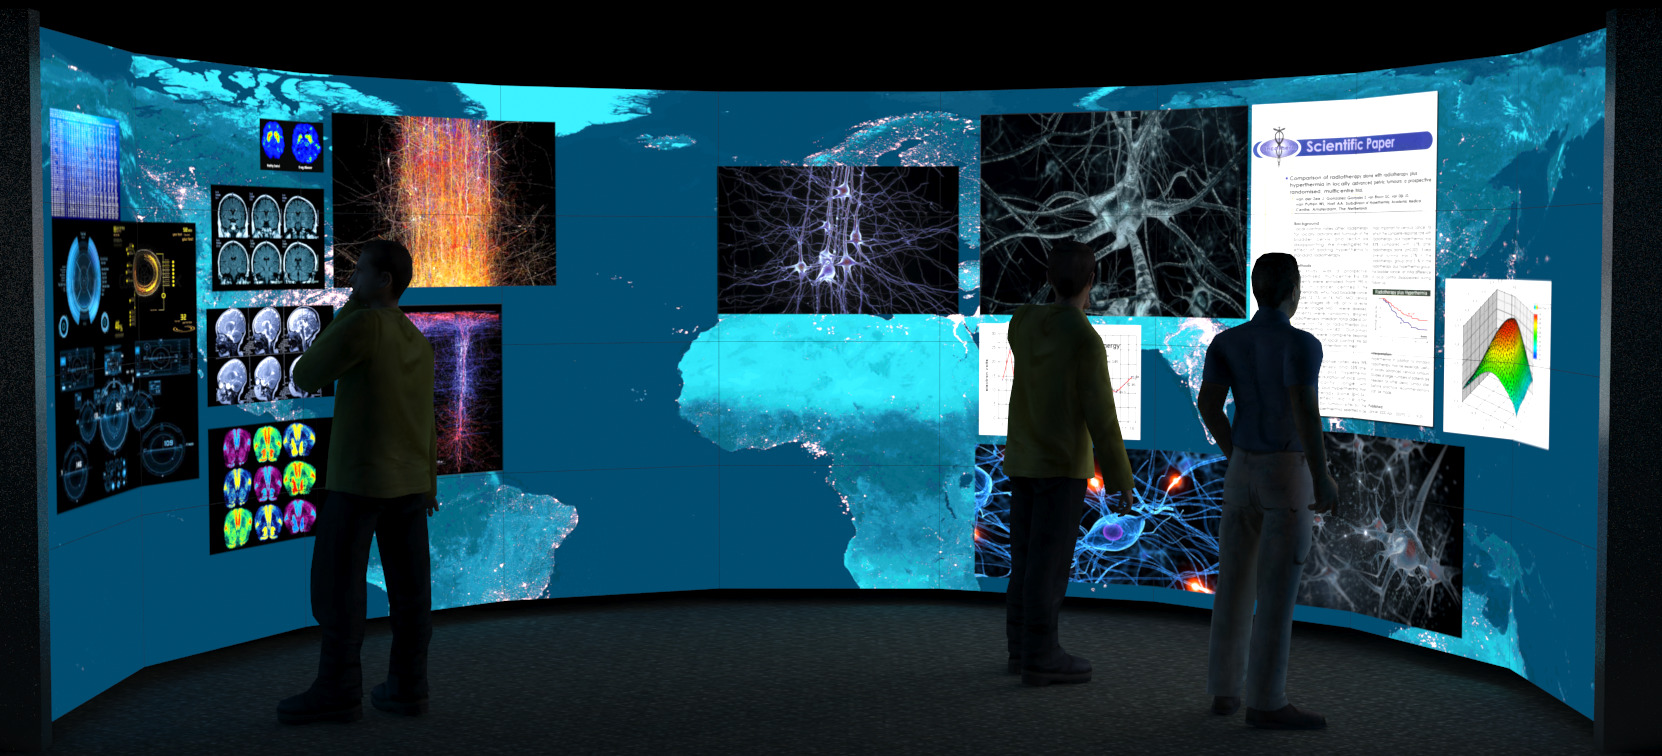
\includegraphics[width=\columnwidth]{images/opendeck}
  \caption{\label{fOpenDeck}OpenDeck concept rendering}
\end{figure}

The OpenDeck will provide a unique environment for the research and development
of new visualization techniques. The main area of research will be mixed reality
systems, such as touch interface implementation in an immersive environment, and
the transition from 2D content to full immersion. The OpenDeck immersive
infrastructure with multitouch will open a set of questions along immersive
touch user interfaces, transitions and mixing of monoscopic to immersive usage,
the combination of tracked and touch devices, multi-user immersion, latency for
remote immersive rendering as well as multi-site collaboration.

\subsection{Tide}

Tide (Tiled Interactive Display Environment) is the software driving the Blue
Brain tiled display walls and OpenDeck. It provides multi-window, multi-user
touch interaction on large surfaces --- think of a giant collaborative
wall-mounted tablet. Tide is a distributed application that can run on multiple
machines to power display walls or projection systems of any size. Its user
interface is designed to offer an intuitive experience on touch walls. It works
just as well on non touch-capable installations by using its web interface from
any web browser. \fig{fTDW} shows Tide on a $4\times 3$ display wall and
\fig{fTideWeb} shows the Tide web interface in a browser.

\begin{figure}[h!t]
  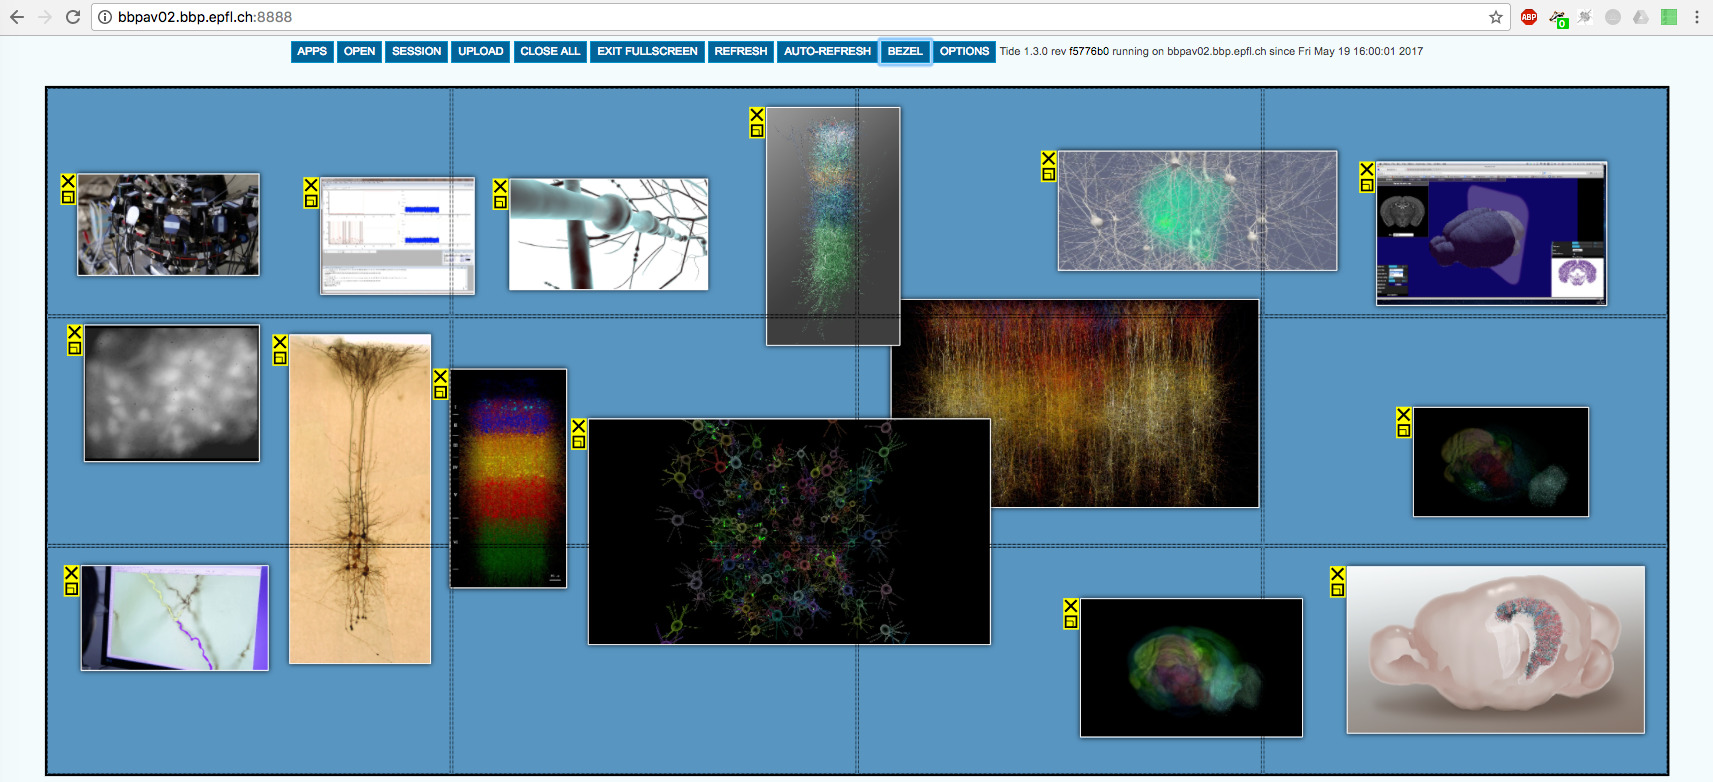
\includegraphics[width=\columnwidth]{images/tideweb}
  \caption{\label{fTideWeb}Tide web interface}
\end{figure}

Compared to other solutions~\cite{Sage,Sage2,DisplayCluster}, the development of
Tide was driven by the need of a stable and easy to use implementation. Tide
supports three types of content: files (high-resolution images, movies, pdfs),
built-in applications (web browser, whiteboard) and remote applications using
the Deflect library (DesktopStreamer, Equalizer-based applications, Brayns).
The multitouch user interface can handle multiple users manipulating different
windows and their content.

\subsection{Deflect}

Deflect is the client library for Tide. It provides an API for pixel streaming
to Tide and for receiving events from Tide. The pixel streaming allows
synchronized parallel streaming from a parallel rendering application as well
as monoscopic and stereoscopic streams. Various events allow the application to
react to multi-touch input from the wall.

Deflect is integrated into the Equalizer parallel rendering
framework~\cite{EMP:09}, enabling transparent usage of Equalizer applications on
Tide walls. Furthermore, the DesktopStreamer application mirrors the desktop of
other machines onto a wall window and allows interaction with the remote
desktop. Other rendering applications, such as our interactive raytracing
engine Brayns~\cite{brayns} are easily integrated with Deflect and Tide.

\section{C++ Messaging and Services}

All Blue Brain applications integrate a messaging framework which allows them
to be used as services in a variety of use cases. For example, the Tide web
server providing the user interface shown in \fig{fTideWeb}, is based on this
messaging solution. Other use cases are remote python APIs, JavaScript user
interfaces and service architectures combining multiple visualization
applications with data providers such as HPC simulations.

The base communication layer ZeroEQ utilizes ZeroMQ as the transport layer, the
ZeroConf protocol for discovery, and our novel ZeroBuf serialization library for
high-performance messaging. A fully integrated HTTP server provides a bridge to
JavaScript, Python and similar environments by implementing REST APIs with JSON
payload. \fig{fUML} shows a class diagram of our messaging solution.

\begin{figure*}[ht]\center
  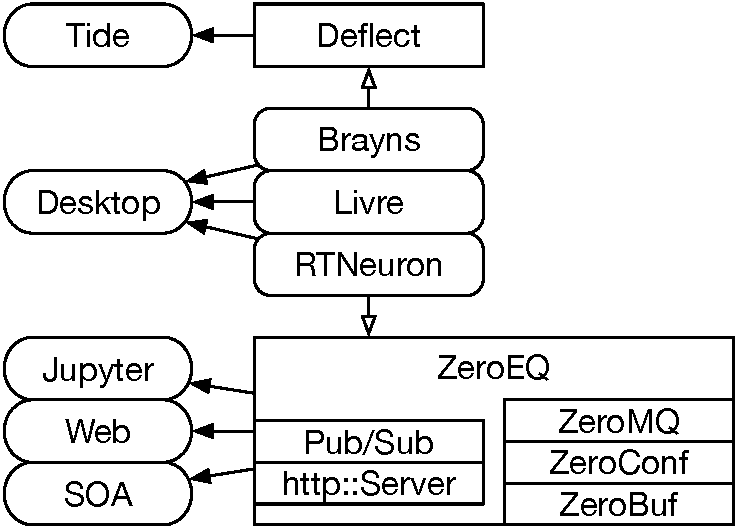
\includegraphics[width=\columnwidth]{images/ZeroMS}
  \caption{\label{fUML}UML Diagram of the main messaging classes}
\end{figure*}


\subsection{ZeroEQ}

ZeroEQ is the base messaging library, wrapping up existing technologies into an
API which is convenient to use and easy to integrate into C++ code. It provides
two messaging services: publish-subscribe and HTTP. For binary and JSON
encodings it relies on a simple \textsf{Serializable} interface, for which
ZeroBuf provides a sample implementation. To facilitate the simple use case of
linking a few applications, ZeroEQ uses the zeroconf protocol to discover and
connect to related applications. For more complex scenarios, explicit
connections are supported.

\subsubsection{Publish-Subscribe}

The publish-subscribe service is implemented in a \textsf{Publisher} and
\textsf{Subscriber} class. It provides event-based messaging, based on a 128-bit
message type with arbitrary payload. The message type is used for message
subscription, filtering and routing. The payload is expected to be uniquely
identified by the message type, that is, all applications agree for the decoding
and semantics of any given message type. The ZeroBuf section outlines how this
is implemented. The underlying transport uses ZeroMQ pub-sub sockets.

The pub-sub service is stateless, that is, applications have no expectation of
when messages are received or who receives published messages. This
communication pattern naturally leads to robust services, since there is no
possiblity for deadlocks or undefined behaviour. The pub-sub API is provided in
two flavors: a simple $pointer \& size$ memory buffer, and a higher level
object-based abstraction. The object-based API is syntactic sugar for the
low-level API, and allows automatic publish and update of objects with a few
lines of code. It uses the \textsf{toBinary()} and \textsf{fromBinary()} methods
of the \textsf{Serializable} interface to call the low-level API.

\begin{lstlisting}[float, caption=Publish-Subscribe Example, label=lPubSub]
zerobuf::render::Camera camera;
zeroeq::Publisher publisher;
zeroeq::Subscriber subscriber;

subscriber.subscribe( camera );

while( rendering )
{
    subscriber.receive( 0 /*ms, poll*/ );
    updateCamera( camera );
    publisher.publish( camera );
    renderFrame( camera );
}
\end{lstlisting}

The example in \lref{lPubSub} shows the integration of camera
synchronization in a visualization application. This example relies on the
builtin zeroconf protocol to connect application instances. Subscribers only
subscribe to events from publishers within the same session. The default
session name is the user name, and can be customized using an environment
variable or non-default constructor. Similarly, the subscriber can subscribe by
session or address. \lref{lPubSubExp} illustrates an explicitly addressed
subscription. Notice that the subscriber uses the publisher URI, which will
contain the concrete port chosen for the publisher.

\begin{lstlisting}[float, caption=Explicit Addressing,label=lPubSubExp]
zeroeq::URI uri( "tcp://localhost" );
zeroeq::Publisher publisher( uri, zeroeq::NULL_SESSION ); // deactivate zeroconf
zeroeq::Subscriber subscriber( publisher.getURI( )); // use concrete port
\end{lstlisting}

Subscribers are derived from a \textsf(Receiver) base class, which is shared
with the http server. All receivers can share their \textsf{receive()}
operation at construction time, that is, the blocking receive operation applies
to all receivers in the shared group. \lref{lSubShare} shows an example of
selectively receiving different updates on different input sockets.

\begin{lstlisting}[float,caption=Subscriber Sharing, label=lSubShare]
zeroeq::Subscriber local( zeroeq::URI( "localhost:29387" ));
zeroeq::Subscriber global( local );

local.subscribe( colorMap );
global.subscribe( camera );

while( true )
    local.receive(); // updates colorMap and camera
\end{lstlisting}

\subsubsection{HTTP Server}

The http server is built using cppnetlib~\cite{cppnetlib} for the transport and
http protocol handling. It supports all standard http verbs (GET, POST, PUT,
PATCH, DELETE). It is a \textsf{zeroeq::Receiver}, that is, it can share its
\textsf{receive()} update operation with other subscribers and http servers.
Unlike a subscriber, the http server follows the HTTP request-reply semantics,
that is, a request received by a server has to be followed directly by its
reply. To allow asynchronous request processing, the return value from the
request handler is a \textsf{std::future} which is retrieved from an internal
thread, thus allowing the application to continue operations.

The http server is introspectable, it allows querying the available endpoints
(objects) and the JSON schema~\cite{jsonschema} for each endpoint.
\lref{lhttpReg} shows an excerpt of the Tide registry, and \lref{lhttpSchema} an
excerpt of the schema for one of the exposed objects. This REST API is used by
the Tide web interface from Javascript and to generate remote python APIs.

\noindent\begin{minipage}[b][][b]{.48\textwidth}
\begin{lstlisting}[caption=HTTP Server Registry, label=lhttpReg]
> GET /registry HTTP/1.0
{
[...]
   "tide/open" : [ "PUT" ],
   "tide/options" : [ "GET", "PUT" ],
   "tide/resize-window" : [ "PUT" ],
[...]
}
\end{lstlisting}
\end{minipage}\hfill
\begin{minipage}[b][][b]{.48\textwidth}
\begin{lstlisting}[caption=Object JSON Schema, label=lhttpSchema]
> GET /tide/options/schema HTTP/1.0
{
[...]
    "properties": {
        "alphaBlending": {
            "type": "boolean"
        },
[...]
}
\end{lstlisting}
\end{minipage}

\subsection{Remote Python API}

The remote python API provides easy to use access to remote applications using
the http server. It integrates two features: generic code generation for the
REST API exposed by the application, and automatic resource allocation and
application launch.

The generic code generation is implemented in a pure python module, which has
no dependency to the interfaced C++ application. It queries the http server and
generates a python API for all exposed objects. This API can then be
conveniently used in python to remote control the application.

Access to the application is established either through an explicit connection
of a pre-launched application, or via a resource allocator. The allocator hides
the details of allocating a resource, e.g. using a scheduling system like
slurm, launching and connecting to the launched application from the python
programmer.

\section{Rendering Applications}

The rendering applications form the backbone of our ecosystem.

\subsection{Interactive Raytracing}

\subsection{OpenGL Parallel Rendering}

\subsection{Out-of-Core Volume Rendering}

Real-time rendering of volumetric data suffers from the curse of
dimensionality. The data size of regular grids increases cubically as the number
of dimensions increase. To render such data interactively, out-of-core (OOC)
storage using multi-resolution algorithms are commonly employed.

Livre is an interactive volume rendering engine available under a permissive
open source license. Our main contribution are: an state-of-the-art
implementation of an octree-based level-of-detail selection, a task parallel
rendering pipeline, a multi-GPU based parallel rendering engine, and an easily
extensible renderer through the use of plugin data sources. Furthermore we
propose to create volume representations of different input data using
on-the-fly, interactive transformations of the data, skipping costly
preprocessing steps.

Our system brings together state-of-the art algorithms to create a volume
rendering engine capable of handling extremely high-resolution volumes using a
high degree of parallelism, both on a single system as well as in a distributed
cluster. We employ a GPU-based ray casting algorithm to compute the radiance
absorption of the given volumetric data. The computation is executed per pixel
on the pixel shader hardware of the GPU.

In our out-of-core data access layer, multi-resolution data is represented as an
octree data structure. This representation accelerates the selection of the
proper level-of-detail and to track the status of the LODs (in CPU memory, in
GPU memory, not loaded). While rendering, view-based LOD selection is performed
using the on the screen-space-error (SSE)~\cite{guthe2004} technique. According
to the requested maximum SSE, the selected LODs represent the given volume the
best on the screen.

The creation of volume bricks, their upload to the GPU and the rendering are
executed in separate tasks. These tasks run asynchronously, that is, they do not
block each other. This is particularly important for the render thread, which
has to react to user input as quickly as possible to reduce input latency, and
renders at interactive frame rates. The data loader thread can take seconds to
generate the brick, for example in the field voxelization data source when
sampling millions of events.

Livre uses a plugin mechanism to access the volume data. In this mechanism, data
sources are implemented as shared libraries and are loaded on application
startup based on the URI of the input data. Loading the shared libraries on
runtime allows to add third-party data loaders to an existing Livre application
by simply placing them into the shared library directory. Data sources have to
provide the requested volume bricks, that is, there is no defined file format or
even requirement to read the input data from a file system. This flexibility of
the plugin approach lead to novel volume rendering use cases, where volume
representations are created on the fly from different input data sets.


%----------------------------------------------------------------------
\section{Discussion and Conclusion}
%----------------------------------------------------------------------
\label{sec:conclusions}

%----------------------------------------------------------------------
\section*{Acknowledgments}
%----------------------------------------------------------------------
This publication was supported by the Blue Brain Project (BBP), the Swiss
National Science Foundation under Grant 200020-129525, the King Abdullah
University of Science and Technology (KAUST) through the KAUST-EPFL alliance for
Neuro-Inspired High Performance Computing, the Spanish Ministry of Science and
Innovation under grant (TIN2010-21289-C02-01/02), the Cajal Blue Brain Project,
Hasler and HBP.


\bibliographystyle{abbrv}
\bibliography{references/references}

% that's all folks
\end{document}
